% ----------------------------------------------------------
% Subseção Consciência
% ----------------------------------------------------------
\subsection{Consciência}
Como visto na seção do teorema central do limite, um momento lógico é formado por divisão e subdivisões lógicas, como são as subunidades de espaço ou tempo. Um momento lógico pode ser representado por suas subunidades ou por sua unidade.

\begin{figure}[H]
\caption{Intervalos lógicos}
\label{fig:2_consciousnesses_in_all_unconscious}
\centering
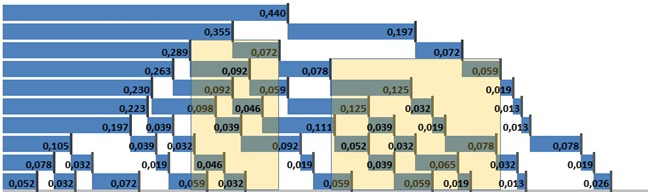
\includegraphics[scale=1]{sections/images/2_consciousnesses_in_all_unconscious.jpg}
\floatfoot{Exemplo de abrangência de dois intervalos lógicos.}%\footnotemark}
\end{figure}
%\footnotetext{Fonte: note}

A consciência são os momentos lógicos de um intervalo representados em suas unidades.

\begin{figure}[H]
\centering
	\begin{subfigure}[H]{.8\linewidth}
	\centering
	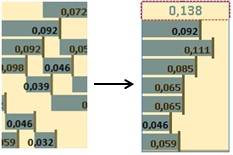
\includegraphics[width=.6\linewidth]{sections/images/first_consciousness.jpg}
	\caption{}
	\label{fig:first_consciousness}
	\end{subfigure}
%\hfill
	\begin{subfigure}[H]{.8\linewidth}
	\centering
	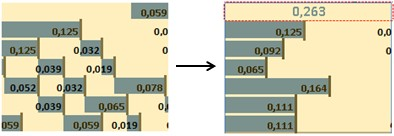
\includegraphics[width=1\linewidth]{sections/images/second_consciousness.jpg}
	\caption{}
	\label{fig:second_consciousness}
	\end{subfigure}%
\caption{Intervalos conscientes}

\floatfoot{Exemplo de dois intervalos conscientes, momentos lógicos como unidades de negação.} %\protect\footnotemark}
\end{figure}
%\footnotetext{Note}

Pode ser observado na Tabela \ref{tab:10000_all} que a probabilidade de 99,99\% das amostras, que aumentam em quantidade a medida que crescem os momentos lógicos, tendem a estar cada vez mais ao centro do intervalo lógico, sendo que essa centralização tende ao infinito.

\begin{figure}[H]
\caption{Centralização de 99,99\% das amostras}
\label{fig:centering_of_99_range}
\centering
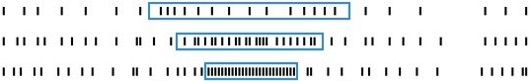
\includegraphics[scale=1]{sections/images/centering_of_99_range.jpg}
\floatfoot{Tendência de centralização do range de 99,99\% das amostras.}%\footnotemark}
\end{figure}
%\footnotetext{Fonte: note}

A Figura \ref{fig:unconsciousness_consciousness_consciousness_nested} também exemplifica bem essa centralização de 99.99\% das amostras na parte da figura nomeada \textbf{Consciência}. Nela é possível ver que as extremidades que em dado momento estiveram dentro desse range de 99.99\% passam a ter uma relevância lógica cada vez mais próxima de zero à medida que crescem os momentos lógicos. Porém, o que não é tão relevante na parte da Figura nomeada \textbf{Consciência} (uma consciência maior e mais abrangente), continua sendo extremamente relevante à \textbf{Consciência aninhada} (consciências menores). É análogo ao que acontece no corpo humano, não é observado pela consciência humana às mudanças de todas as células do corpo ou ainda de muitos órgãos, porém esses outros níveis de abstração sofrem a mesma evolução da negação de si. A contínua expansão centralizada da \textbf{Consciência} e da \textbf{Consciência aninhada} sugerem a formação dos chamados buracos negros, detalhados mais a frente. Essas características também sugerem que buracos negros podem conter outros buracos negros.

\begin{figure}[H]
\caption{Consciência e Consciência aninhada}
\label{fig:unconsciousness_consciousness_consciousness_nested}
\centering
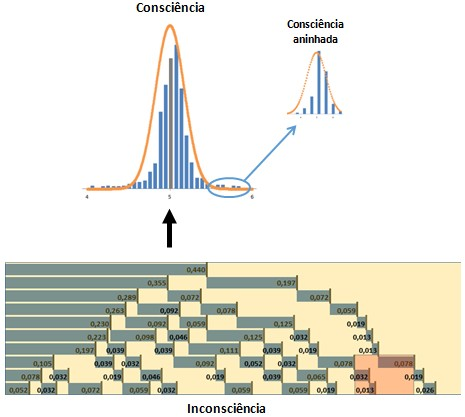
\includegraphics[scale=1]{sections/images/unconsciousness_consciousness_consciousness_nested.jpg}
\floatfoot{Esboços de histogramas que exemplificam a consciência e consciência aninhada.}%\footnotemark}
\end{figure}
%\footnotetext{Fonte: note}

A consciência é o conjunto dos momentos lógicos de um intervalo. É o aspecto da lógica que unifica as amostras desses momentos, ou seja, é a lógica que abstrai muitos em um, muitas subunidades em uma unidade por momento lógico, podendo essa unidade ser uma subunidade de uma unidade superior. Todos os aspectos listados abaixo são inerentes a abstração da lógica chamada consciência.

\subsubsection{Infinito}
Um dos aspectos mais importantes que a negação do nada traz (negação de si), é o infinito. E um dos aspectos mais importantes do infinito é que as possibilidades lógicas encontradas em um intervalo lógico superior podem também ser encontradas em intervalos lógicos inferiores. A chance de ciclos de possibilidades idênticos é uma das infinitas possibilidades do infinito. Ou seja, todo intervalo lógico é um começo, assim a criatura pode ser o criador daquele que o criou em outr fluxo lógico. Não há fim, não há meio, apenas infinitos começos. Isso fundamenta como uma lógica complexa como a consciência explica a lógica primordial, uma vez que não é preciso voltar ao primeiro momento lógico de todo o intervalo para observá-lo, toda negação de um intervalo  ou subintervalo lógico é seu primeiro momento lógico.

\subsubsection{Tempo}
O tempo é a adição de novos momento lógicos à medida que prossegue a negação desses momentos.  Essas mudanças são acumulativas e o momento lógico futuro é gerado pela negação do momento presente e somado a este tornando a consciência diferente.

\begin{figure}[H]
\caption{Tempo}
\label{fig:consciousness_time}
\centering
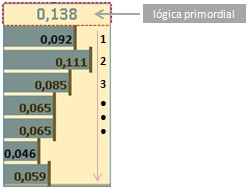
\includegraphics[scale=1]{sections/images/consciousness_time.jpg}
\floatfoot{Progressão do tempo conforme os momentos lógicos avançam.}%\footnotemark}
\end{figure}
%\footnotetext{Fonte: note}

\subsubsection{Espaço}
O espaço é a relação da proporção dos intervalos dos momentos lógicos. A proporção da fração lógica (intervalo azul) com a unidade lógica (intervalo cinza), da unidade com a fração lógica e da diferença de entre as frações lógicas.

\begin{figure}[H]
\caption{Espaço}
\label{fig:consciousness_space}
\centering
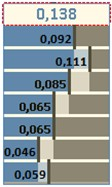
\includegraphics[scale=1]{sections/images/consciousness_space.jpg}
\floatfoot{Relação da proporção dos intervalos dos momentos lógicos.}%\footnotemark}
\end{figure}
%\footnotetext{Fonte: note}

\subsubsection{Gravidade}
A gravidade é um aspecto probabilístico da distribuição amostral de uma população, como previsto pelo teorema central do limite. Esse teorema afirma que a distribuição amostral de uma população se aproxima de uma distribuição normal à medida que o tamanho das amostras aumenta, o que tende probabilisticamente à centralização infinita das amostras conforme os momentos lógicos progridem. A atração do amor, a gravidade que atraem os objetos à terra e a terra ao sol são sinônimos deste mesmo aspecto.

\begin{figure}[H]
\caption{Gravidade}
\label{fig:consciousness_gravity}
\centering
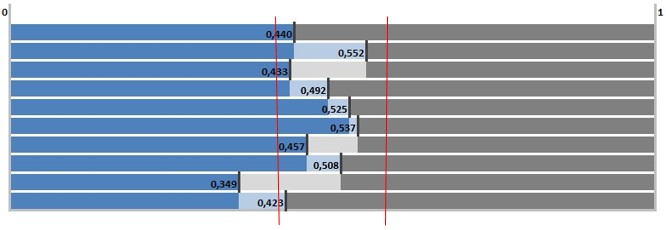
\includegraphics[scale=1]{sections/images/consciousness_gravity.jpg}
\floatfoot{Centralização infinita das amostras conforme os momentos lógicos progridem.}%\footnotemark}
\end{figure}
%\footnotetext{Fonte: note}

\subsubsection{Matéria escura e energia escura}
Quanto maior o número e mais próximas as amostras estão da mediana, mais amostras farão parte dos 99,99\% e mais amostras também estarão nos 0,01\%, conforme a Tabela \ref{tab:10000_all}. Assim, a observação desses 0,01\% passa a ser cada vez mais difícil, pois sua relevância consciente passa a ser cada vez mais próxima de zero. É importante notar também que a medida que os 99,99\% aumentam em número de amostras, menos relevante cada nova amostra será dentro desse conjunto. Um em cem mais relevante do que um em mil. 

\begin{figure}[H]
\caption{Analogia da matéria escura e energia escura}
\label{fig:consciousness_dark_matter_dark_energy}
\centering
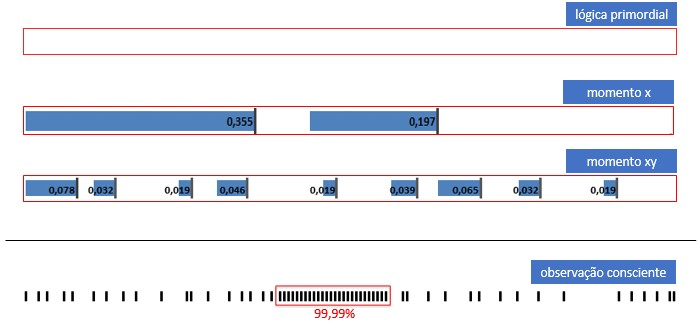
\includegraphics[scale=1]{sections/images/consciousness_dark_matter_dark_energy.jpg}
\floatfoot{Fenômenos antevistos ou conjecturados pela consciência.}%\footnotemark}
\end{figure}
%\footnotetext{Fonte: note}

\subsubsection{Antimatéria}
Independente do intervalo observado (análogo à bytes, kilobytes, prótons, elétrons etc.), que são contextos lógicos de observação e/ou utilização consciente, este pode estar com sua maior concentração de amostras no sentido da mediana, o que é o sentido provável conforme os números de amostras crescem em um intervalo, conforme teorema central do limite. Essas amostras também podem estar com sua concentração no sentido oposto a mediana, porém com uma ocorrência probabilística cada vez menos conforme as amostras aumentam. Na Figura \ref{fig:consciousness_concentration_of_opposite_samples} é exibido dois intervalos idênticos com suas amostras com concentrações opostas.

\begin{figure}[H]
\caption{Parte de um intervalo idêntico com suas concentrações de amostras opostas}
\label{fig:consciousness_concentration_of_opposite_samples}
\centering
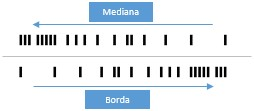
\includegraphics[scale=.8]{sections/images/consciousness_concentration_of_opposite_samples.jpg}
\floatfoot{Parte de um intervalo idêntico distribuídos de formas opostas.}%\footnotemark}
\end{figure}
%\footnotetext{Fonte: note}

O merge ou soma dos intervalos opostos da Figura \ref{fig:consciousness_concentration_of_opposite_samples} os tornaria um intervalo simétrico, ou seja, não estaria em nenhum dos sentidos.
Na Figura \ref{fig:consciousness_concentration_of_opposite_samples_within_range} é exibido um intervalo consciente completo com suas concentrações de amostras sentido à mediana e outro idêntico, mas com suas concentrações sentido às bordas do intervalo.

\begin{figure}[H]
\caption{Intervalos conscientes com suas concentrações de amostras opostas}
\label{fig:consciousness_concentration_of_opposite_samples_within_range}
\centering
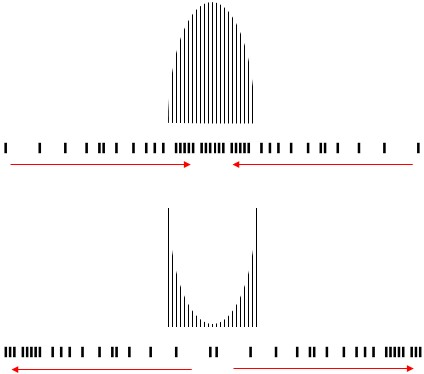
\includegraphics[scale=.8]{sections/images/consciousness_concentration_of_opposite_samples_within_range.jpg}
\floatfoot{Intervalos conscientes completos e idênticos distribuídos de formas opostas.}%\footnotemark}
\end{figure}
%\footnotetext{Fonte: note}

\subsubsection{Buraco negro}
Assim como a gravidade o buraco negro é um aspecto probabilístico da distribuição amostral de uma população, como previsto pelo Teorema Central do Limite. Quanto mais momentos lógicos, mais amostras, o que tende a centralizar cada vez mais amostras da consciência em uma proporção cada vez menor do intervalo lógico. Essa proporção do intervalo lógico cada vez menor tende ao infinito assim como a quantidade de amostras crescentes que ela envolve, ou seja, um alto volume de amostras em uma proporção inobservável a certas abstrações de consciência. Com essa observação é possível observar que as consciências tendem a se concentrar em intervalos infinitamente menores à medida que crescem, portanto a morte lógica ou consciente é apenas a incapacidade de observação de proporções infinitamente pequenas.

\begin{figure}[H]
\caption{Buraco negro}
\label{fig:consciousness_black_hole}
\centering
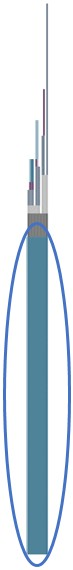
\includegraphics[scale=1]{sections/images/consciousness_black_hole.jpg}
\floatfoot{Centralização infinita das amostras em uma proporção centralizada cada vez menor.}%\footnotemark}
\end{figure}
%\footnotetext{Fonte: note}

\subsubsection{Coexistência inferida}
A tendência probabilística descrita pelo teorema central do limite faz com que a população concentre uma frequência menor de amostras em suas extremidades que vai aumentando gradualmente conforme se aproxima da mediana. A frequência de amostras dispostas desta forma torna as interações conscientes mais semelhantes em conjuntos de amostras adjacentes. Assim, ao comparar a frequência de um conjunto de amostras próximo à mediana com um conjunto de amostras mais próximo da extremidade de uma grande população, probabilisticamente haverá uma grande discrepância em suas frequências, ou seja, em um mesmo intervalo haverá mais amostras no conjunto próximo à mediana. Essa observação mostra que conjuntos ou intervalos de frequências adjacentes são mais parecidos do que conjuntos distantes. 

Para exemplificar, um ser humano tem sua consciência formada por conjuntos distantes como estrelas, galáxias etc., os quais são conjuntos de frequências bem distintas das que estão nas proximidades da mediana, que são o núcleo dessa consciência e, portanto, esses conjuntos distantes além de terem frequências bem diferentes sofrem menos interações conscientes, uma vez que, probabilisticamente, a concentração das novas amostras estão próximos aos conjuntos adjacentes à mediana, ou seja, esses conjuntos próximos à mediana têm frequências parecidas e sofrem maior interação. No caso de um ser humano essas iterações são representados pelas iterações que um ser humano tem com outro.  

Ao observar uma consciência humana (A), a qual representa todo o intervalo em questão, pode-se observar que a interação do núcleo (conjunto de amostras próximo à mediana) com os conjuntos adjacentes semelhantes, por exemplo, a interação do ser humano (A) como o ser humano (B) observado pela consciência do primeiro, faz com que o ser humano (A) tenha uma percepção do ser humano (B) como uma riqueza menor de detalhes, uma vez que o ser humano (B) não é o núcleo dessa consciência e por isso recebe um volume menor de novas amostras. Por outro lado, ao observar um intervalo semelhante logicamente, porém onde o ser humano (B) é o núcleo consciente, este de forma semelhante observaria o ser humano (A) com uma riqueza menor de detalhes. Assim, a interação do ser humano (A) e (B) são equivalentes logicamente, sendo núcleo ou não de uma consciência. Logo, para o ser humano (A), núcleo da consciência, a observação do ser humano (B) é implícita, ou seja, é subentendida como equivalente a observação contraria, do ser humano (B) para o (A). A interação lógica entre conjuntos de um intervalo pode acontecer de forma equivalente independente de qual conjunto é o núcleo consciente. 

\begin{figure}[H]
\caption{Conjuntos de frequências de um intervalo}
\label{fig:consciousness_inferred_coexistence}
\centering
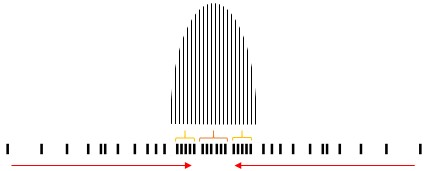
\includegraphics[scale=1]{sections/images/consciousness_inferred_coexistence.jpg}
\floatfoot{Diferentes frequências de um intervalo e a redução de detalhes dos conjuntos semelhantes proxímos à mediana em relação ao conjunto central.}%\footnotemark}
\end{figure}
%\footnotetext{Fonte: note}
